
%
%  $Description: Author guidelines and sample document in LaTeX 2.09$ 
%
%  $Author: ienne $
%  $Date: 1995/09/15 15:20:59 $
%  $Revision: 1.4 $
%

\documentclass[times, 10pt,twocolumn]{article} 
\usepackage{paper}
\usepackage{times}
\usepackage{graphicx}
\usepackage{float}

%\documentstyle[times,art10,twocolumn,latex8]{article}

%------------------------------------------------------------------------- 
% take the % away on next line to produce the final camera-ready version 
\pagestyle{empty}

%------------------------------------------------------------------------- 
\begin{document}

\title{Citi Bike Usage Balancing through Congestion Pricing}

\author{Paul Griffioen\\Dept. of Electrical and Computer Engineering\\Carnegie Mellon University\\ pgriffi1@andrew.cmu.edu\\
% For a paper whose authors are all at the same institution, 
% omit the following lines up until the closing ``}''.
% Additional authors and addresses can be added with ``\and'', 
% just like the second author.
\and
Anthony Jin\\Dept. of Electrical and Computer Engineering\\Carnegie Mellon University\\xiaoxiaj@andrew.cmu.edu\\
}

\maketitle
\thispagestyle{empty}

%------------------------------------------------------------------------- 
\Section{Abstract}

The issue of congestion in bicycle sharing systems is prevalent in many cities. This project proposes an incentive-based pricing scheme for New York City's Citi Bike system that minimizes bicycle congestion. It approaches bicycle sharing systems from a network perspective, analyzing and optimizing the network by providing monetary incentives to users with the intent of modifying network properties. These monetary incentives are part of a much larger optimization problem designed to minimize both user dissatisfaction and bicycle congestion. To demonstrate the effectiveness of this approach, the Citi Bike system is modeled and simulated using MATLAB, where monetary incentives are given to users such that user dissatisfaction and bicycle congestion are minimized.

%------------------------------------------------------------------------- 
\Section{Introduction and Motivation}

The Citi Bike system, located in New York City, is one of many bicycle sharing systems that exist in the world. Since users unlock a bike at one station and drop it off at another station, bikes tend to follow unidirectional flows at various times of the day. As a result, some stations have few to no bikes at them while others are completely full.

This unidirectional flow of bikes frustrates users who would like to pick up a bike from an empty station or drop off a bike at a full station. As a result, this project seeks to address the issue of system congestion through a pricing scheme based on the optimization of network structure and dynamics. In addition, alteration of the network topology to reduce congestion will be explored through optimal placement of nodes (stations). Looking at the problem from a network perspective is a unique approach that has not been considered with previous work. In the end, this project seeks to analyze the Citi Bike network and to minimize congestion by modifying its structure through changing people's incentives.

%------------------------------------------------------------------------- 
\Section{Previous Work}

Previous work has taken many viewpoints to solve the bike sharing congestion problem. The work in \cite{incentives} proposes a dynamic incentives system that involves future traffic prediction, truck-based re-positioning policies, and schema to compute monetary incentives for users. The authors in \cite{redistribution} use a similar approach, combining staff-based dynamic vehicle distribution and real-time pricing incentives for customers. In contrast, \cite{management} and \cite{redistribution} look at the inventory management of individual bike-sharing stations and formulate appropriate convex optimization problems. Similar to the aforementioned approaches, this project will address the congestion problem as a convex optimization problem and introduce a congestion-based pricing scheme to modify user incentives. Unlike prior work, however, it takes a network standpoint and models the Citi Bike system as a dynamic network.

%------------------------------------------------------------------------- 
\Section{Approach}

The Citi Bike network is built using available data from Citi Bike's website \cite{dataset}. The nodes represent different bike stations and the weighted links represent the number of trips made from one station to another in a certain time period $t$. We are also interested in a few node and edge attributes: each node (bike station) has an identification number, latitude and longitude, maximum capacity, and current number of stored bikes; meanwhile, each edge (bike trip) has a bike identification number and user age and subscription type. These attributes are used as inputs in the convex optimization problem for the incentive-based pricing scheme.

The trip data in \cite{dataset} does not include explicit information about the addition or removal of bikes to the system or the transfer of bikes by truck from one station to another. Consequently, this project can only analyze bike trips from one station to another. In addition, there is no information about the number of bikes at particular stations at specific points in time. As a result, an initialization procedure is used to infer this information. 

\subsection{Parameters}

To provide accurate monetary incentives to users, a convex optimization problem is formulated that seeks to minimize bicycle congestion and user dissatisfaction. The following terms, which are applied in a certain time interval $t$, are used in the formation of the convex optimization problem. $u = \{u_1, u_2, ..., u_n\}$ represents the set of $n$ users in the Citi Bike network, $A_u$ represents the age of user $u$, and $r_u$ represents the maximum distance user $u$ is willing to walk. $s = \{s_1, s_2, ..., s_m\}$ is the set of $m$ bike stations in the Citi Bike network, and $s_{pu}$ and $s_{du}$ represent user $u$'s intended pick-up and drop-off stations, respectively. As a result, $d_{pu} = \{d_{pu1}, d_{pu2}, ..., d_{pum}\}$ and $d_{du} = \{d_{du1}, d_{du2}, ..., d_{dum}\}$ denote the set of distances between the set of all stations $s$ and station $s_{pu}$ or $s_{du}$, respectively. $G_s$ represents the congestion level at station $s$, where $C_s$ denotes the maximum capacity at station $s$, $v_s$ denotes the current number of bikes at station $s$, and $o_s$ and $i_s$ denote the out-degree and in-degree of station $s$, respectively. $k$ is a constant that weights the impact of the out-degree and in-degree on the congestion level. Next, $s_{pu*} = \{s_{pu1}, s_{pu2}, ...\}$ and $s_{du*} = \{s_{du1}, s_{du2}, ...\}$ represent user $u$'s set of candidate stations for pick-up and drop-off, respectively. $d_{pu*} = \{d_{pu*1}, d_{pu*2}, ...\}$ and $d_{du*} = \{d_{du*1}, d_{du*2}, ...\}$ denote the set of distances between the set of stations $s_{pu*}$ and station $s_{pu}$ or between the set of stations $s_{du*}$ and station $s_{du}$, respectively. In addition, $p_u = \{p_{u1}, p_{u2}, ..., p_{max}\}$ represents the ordered set of payments offered to user $u$ where $p_{max}$ is the same for all users. $B$ represents the current budget for the entire Citi Bike network, and $S_u$ is a variable that equals $1$ if user $u$ is a subscriber and equals $0$ otherwise. $D_u$ denotes the dissatisfaction of user $u$, and $c_3$ is a constant that weights how important a user's age is in their dissatisfaction for walking from one station to another. $c_1 = \{c_{11}, c_{12}, ...\}$ and $c_2 = \{c_{21}, c_{22}, ...\}$ denote two sets of constants associated with the sets $d_{pu*}$ and $d_{du*}$, respectively, that weight the likelihood of user $u$ choosing to walk to a different station. Also, $a_j$ is a constant that weights the likelihood of user $u$ choosing payment option $p_{uj}$. Lastly, $w_1$ and $w_2$ represent constants that weight the importance of minimizing congestion and user dissatisfaction, respectively.

\subsection{Sub-Functions}

\begin{equation}
r_u = f(A_u)
\end{equation}
\begin{equation}
d_{pu} = f(s_{pu}, s)
\end{equation}
\begin{equation}
d_{du} = f(s_{du}, s)
\end{equation}
\begin{equation}
G_s = C_s - v_s + k(o_s - i_s)
\end{equation}
\begin{equation}
s_{pu*} = f(G_s, d_{pu}, r_u)
\end{equation}
\begin{equation}
s_{du*} = f(G_s, d_{du}, r_u)
\end{equation}
\begin{equation}
d_{pu*} = f(s_{pu}, s_{pu*})
\end{equation}
\begin{equation}
d_{du*} = f(s_{du}, s_{du*})
\end{equation}
\begin{equation}
p_u = f(B, n, d_{pu*}, d_{du*}, A_u, S_u)
\end{equation}
\begin{equation}
p_{max} = B/n
\end{equation}
\begin{equation}
D_u = c_3A_u(c_1d_{pu*} + c_2d_{du*}) + G_s - \sum_{j=1}^{m}a_jp_{uj}
\end{equation}

These sub-functions are primarily used to compute the bicycle congestion level and the user dissatisfaction at a particular station. The congestion level is simply equal to the station's number of currently open docks ($C_s - v_s$) plus an estimate as to how many docks will be taken or will be freed in the near future ($k(o_s - i_s)$). The user dissatisfaction is designed so that dissatisfaction increases with congestion level ($G_s$) and the distance the user has to walk to modify his or her original route ($c_3A_u(c_1d_{pu*} + c_2d_{du*})$). User dissatisfaction decreases with respect to the monetary incentive the user receives ($\sum_{j=1}^{m}a_jp_{uj}$).

\subsection{Objective Function}

\begin{equation}
w_1\sum_{j=1}^{m}\min{|\frac{1}{2}C_s - v_s|} + w_2\min{\sum_{u=1}^{n}D_u}
\end{equation}

The objective function is designed such that overall user dissatisfaction is minimized ($w_2\min{\sum_{u=1}^{n}D_u}$). It is also designed so that each station is as close to half full as possible ($w_1\sum_{j=1}^{m}\min{|\frac{1}{2}C_s - v_s|}$). By designing the objective function in this manner, both user dissatisfaction and bicycle congestion for the Citi Bike system will be minimized.

\subsection{Constraints}

\begin{equation}
d_{pu*} \leq r_u
\end{equation}
\begin{equation}
d_{du*} \leq r_u
\end{equation}
\begin{equation}
v_s \leq C_s
\end{equation}
\begin{equation}
p \geq B/n
\end{equation}
\begin{equation}
\textnormal{all parameters except } G_s \textnormal{and } D_u \geq 0
\end{equation}

%Lastly, the convex optimization problem is formulated in the form of an objective function with constraints. First, we define a few parameters: denote the m stations in the Citi Bike network by the set S = {s1, s2, ... sm}, the maximum bike docks by Cs and the number of bikes available at time t at station s by v(s,t). Assume that a user u with subscription type S and age A intends to pick up a bike from station s(u,1) and head towards station s(u,2). As an attempt to influence the user's decision, the incentive system will suggest two lists of alternative stations, s(*,1) and s(*,2), with associated monetary incentives p*. %p* belongs to P, where P = {pmin, p2, ..., pmax} is a set of fixed prices. A budget B is allocated for the system for a time itnerval t. Lastly, ru represents the maximum distance u is willing to walk.
%
%These parameters are then used to define a set of sub functions:
%% bullet points?
%Congestion: Using the difference between the station's in degree and out degree to estimate the expected number of open docks in the future, the congestion level of bike station s is expressed as 
%\centerline{Cg=Cs-v(s,t)+ks(out degree-in degree)}
%
%Alternative Stations: the lists of alternative stations are determined by ru and the distance between the user's intended station and other bike stations in the set S.
%\centerline{if dist(s(u,1,2), si|si belongs to S) <= ru}
%\centerline{si belongs to s(*,1,2)}
%
%Monetary Incentives: the payment for the user is modeled as a function of 
%
%User dissatisfaction: since the incentives system attempts to alternate the user's initial decision, 

%------------------------------------------------------------------------- 
\Section{Experimental Setup and Practical Results}

\subsection{Network Analysis}
Based on the network definition presented in Section 3, a sample dynamic network is constructed to represent bike usage from Thursday to Saturday in a normal week. First, Citi Bike data from the first three days of September 2016 is extracted from the original data set in \cite{dataset} to generate a node table with 583 nodes and an edge list with more than 130,000 edges. Second, the node table and edge list are imported to Gephi as a dynamic network. The Gephi plugin \textit{Geo Layout} is used to arrange the nodes according to their geographic locations, while network properties are dynamically changed by filtering out edges outside a particular time window. In this analysis, the time window for edge filtering is set to one hour.\\

\centerline{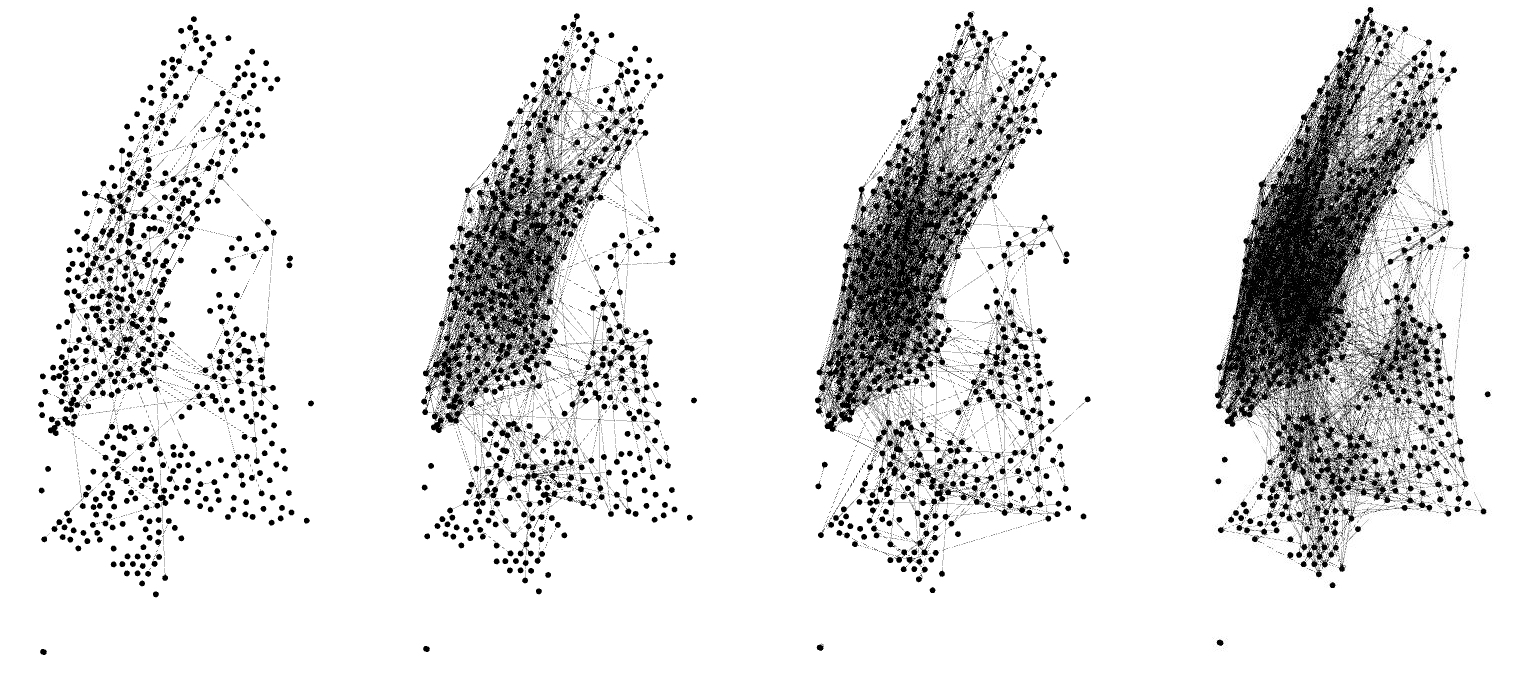
\includegraphics[width=0.5\textwidth]{m2/combined.jpg}}
\centerline{Figure 1: Citi Bike Network on September 1, 2016}
\hfill \break
Figure 1 shows the network at four different time intervals on September 1, 2016. From left to right, the figures represent the network between 1\textsc{am} and 2\textsc{am}, 7\textsc{am} and 8\textsc{am}, 1\textsc{pm} and 2\textsc{pm}, and 7\textsc{pm} and 8\textsc{pm}. Figure 2 illustrates how some of the network properties change over time. Every day, the maximum average node degree is observed between 4\textsc{pm} and 7\textsc{pm}, corresponding to the evening rush hour. On the two weekdays, there is also a secondary peak between 7\textsc{am} and 8\textsc{am}, reflecting the morning rush hour. As expected, this secondary peak is not present on September 3 since it is a Saturday. On the contrary, the network's average path length stays relatively consistent during the day and in the early evening. Bikers seem to take longer trips around midnight and in the morning (between 6\textsc{am} and 7\textsc{am}), while the trips between midnight and 6\textsc{am} tend to be much shorter. As for community structure, the network's modularity and formation of communities exhibit a periodic pattern; during the day, the network has high modularity and the nodes can be grouped into a few communities. At night, the network is less modular and only a handful of nodes can form communities with others.

This network setup has three limitations. First, the congestion level at each station (i.e. maximum capacity versus current number of stored bikes) is not taken into account. Second, the distance between each pair of nodes is assumed to be the same while a more realistic analysis should also take into account the physical distance between stations. Third, only a very small subset of the available data is exploited.

\centerline{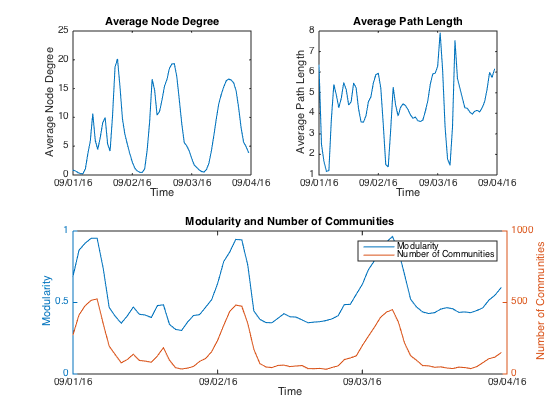
\includegraphics[width=0.5\textwidth]{m2/plotterfigure.png}}
\centerline{Figure 2: Citi Bike Network Properties}

\subsection{Initialization Procedure}
The objective of the initialization procedure is to determine an initial state of the Citi Bike system at any point in time. The procedure starts by identifying a start time and assuming that no bikes are initially in the system. Over a specified time period, bikes are added to the system using incoming trip data for each station and tracked by their identification numbers to determine which station they are at. At the end of this period, it is assumed that all bikes have been added to the system and each station is assigned with an initial number of bikes. Future trip data can now be used to determine the number of bikes at particular stations at any time after the initialization procedure.

\subsection{Citi Bike Network Simulator}

In order to demonstrate whether or not the aforementioned optimization problem results in decongesting the Citi Bike network, a simulator is created using MATLAB. The simulator first uses an entire month's trip data to implement the initialization procedure and estimates how many bikes are at each station. Starting from the next month, trip data entries are stepped through for a user-specified time period. Each entry has a start station and an end station, which correspond to the biker's intended pick-up and drop-off stations defined in the optimization problem. If the congestion level is high for one or both of these intended stations (too empty for pick-up or too crowded for drop-off), the biker will be exposed to random incentives and a list of alternative stations. Currently we assume that the user has a probability of 0.5 to accept the incentives and go to one of the alternative stations, but the probability of choosing a particular station is randomized. For example, if alternative stations s1, s2, and s3 are available, one possibly scenario is that the biker has a probability of 0.1 to choose s1, 0.2 to choose s2, and 0.2 to choose s3. Once the optimization problem is solved, this randomized incentives and probability model will be replaced with more accurate incentives and probability distributions.

After the biker chooses a start and end stations, the state of the Citi Bike system is updated with respect to the number of bikes at each station. Figure 3a shows the state of the Citi Bike system at different times over the course of one day without providing incentives to the bikers and Figure 3b shows the state of the system when the randomized incentives and probability model is implemented. Evidently, the state of the network changes considerably when biker users are exposed to incentives. In light of this, we are confident that successfully solving and implementing the optimization problem will decongest the Citi Bike network.

\centerline{
\includegraphics[width=0.5\textwidth]{m2/blankfigure.png}}
\centerline{Figure 3: Citi Bike Simulator Visualization}

There are a few limitations in this simulator test run: first, there is no information about $10\%$ of the bike stations' maximum capacity, and an estimate must be used. Second, there is no data about bikes being moved to other stations by trucks, and this flow of bikes is unaccounted for. Because of this lack of information, the initial state of the Citi Bike system is slightly inaccurate.

%\centerline{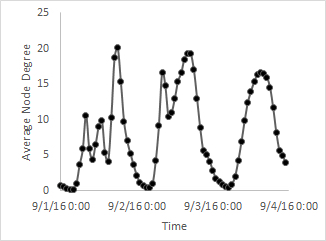
\includegraphics[width=0.4\textwidth]{node_degree.jpg}}
%\centerline{Figure 2: Average Node Degree}
%\vspace{5mm}

%\centerline{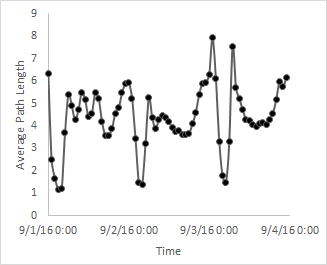
\includegraphics[width=0.4\textwidth]{path_length.jpg}}
%\centerline{Figure 3: Average Path Length}
%\vspace{5mm}

%\centerline{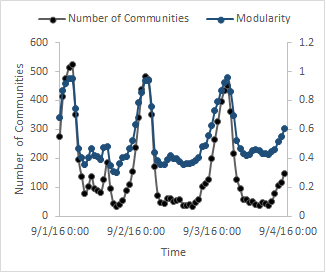
\includegraphics[width=0.4\textwidth]{communities.jpg}}
%\centerline{Figure 4: Modularity and Number of Communities}

%------------------------------------------------------------------------- 
\Section{Conclusion and Short-Term Plans}
This work proposes a framework to decongest the Citi Bike system via convex optimization. After constructing the system as a dynamic network, a MATLAB simulator is used to modify the network's properties using monetary incentives. In addition, the objective function and constraints are defined for the related convex optimization problem. Currently, the framework uses a randomized incentive and probability model to illustrate how the incentives could affect the network. However, the framework will incorporate accurate incentives and probability distributions once the convex optimization problem is solved. In this work, Paul Griffioen focused on developing the MATLAB simulator and Anthony Jin focused on formulating the convex optimization problem.

Future work of this project will focus on solving the proposed optimization problem and integrating the results with the present framework. By Milestone 3, we will finish implementing the decongestion framework with convex optimization and propose the related pricing scheme.
%The basic methodology to construct the Citi Bike network is proposed in this work. Because certain information is not available about the bike stations' capacity, an initialization procedure is also proposed to estimate the number of bikes in the system and at each station. As a preliminary analysis, a sample network is constructed using data between September 1, 2016 and September 3, 2016 to evaluate network properties at different time intervals. In this work, Paul Griffioen extracted network information from the original dataset using MATLAB and Anthony Jin analyzed the network using Gephi.

%The next step of this project is to overcome the limitations of the experimental setup and construct the complete Citi Bike network. By Milestone 2, we will finish the network analysis and begin implementing the pricing scheme.

%------------------------------------------------------------------------- 
%\Section{Overview}
%
%The Citi Bike system, located in New York City, is one of many bicycle sharing systems that exist in the world. Since users unlock a bike at one station and drop it off at another station, bikes tend to follow unidirectional flows at various times of the day. As a result, some stations have few to no bikes at them while others are completely full.
%
%This unidirectional flow of bikes frustrates users who would like to pick up a bike from an empty station or drop off a bike at a full station. As a result, this project seeks to address the bicycle congestion problem by introducing a congestion-based pricing scheme that modifies the incentives of users. It takes a unique approach by solving the congestion problem from a network standpoint as opposed to other viewpoints, such as that presented in \cite{incentives}.
%
%%------------------------------------------------------------------------- 
%\Section{Objectives and Deliverables}
%
%This project seeks to address the issue of system congestion through a pricing scheme based on the optimization of network structure and dynamics. In addition, alteration of the network topology to reduce congestion will be explored through optimal placement of nodes (stations). Large amounts of publicly available data from Citi Bike's website will be used as the main dataset for this project \cite{dataset}. The deliverables for this project include presenting progress, formulating a paper, and participating in a conference-style presentation. In the end, this project seeks to analyze the Citi Bike network and minimize congestion by modifying its structure through changing people's incentives.
%
%%------------------------------------------------------------------------- 
%\Section{Tasks and Timeline}
%
%To accomplish the objectives aforementioned, a timeline with associated tasks is proposed as follows.
%\textit{Network Formulation}: Two to three weeks should be used to build weighted networks of trips for each month using the data found in \cite{dataset}.
%\textit{Network Analysis}: About three weeks should be used to compare the weighted networks in the context of different factors such as weather and seasonality, the time of day, and the day of the week. Additionally, potential user incentives should be identified.
%\textit{Optimization Using Congestion-Based Pricing Scheme}: The congestion-based pricing scheme will take four to five weeks to develop and will deploy the identified user incentives. Specifically, the scheme will feature a user incentive model based on the mathematical models proposed in \cite{incentives} and \cite{redistribution}. In addition, a convex optimization problem will be formulated to account for related objective functions (i.e. minimizing congestion) and constraints (i.e., cost of operation) \cite{sharing} \cite{management}. Ultimately, this scheme aims to optimize the existing network by changing its weights and decreasing congestion.
%\textit{Optimization of Network Topology}: If time permits, an additional task is to examine the topology of the existing network and make appropriate changes to its physical structure by optimizing the placement of nodes.
%
%%------------------------------------------------------------------------- 
%\Section{Conclusion}
%
%This project aims to optimize the Citi Bike network via a congestion-based pricing scheme. Specifically, this scheme will change user incentives and will consequently modify the network's weights while minimizing congestion.

%------------------------------------------------------------------------- 
\nocite{ex1,ex2}
\bibliographystyle{paper}
\bibliography{paper}

%\begin{thebibliography}{}
\begin{thebibliography}{}\setlength{\itemsep}{-1ex}\small

\bibitem{incentives}
A. Singla, M. Santoni, G. Bartok, P. Mukerji, M. Meenen, and A. Krause. "Incentivizing Users for Balancing Bike Sharing Systems." \textit{AAAI}, pp. 723-729, 2015.

\bibitem{redistribution}
J. Pfrommer, J. Warrington, G. Schildbach, and M. Morari. "Dynamic Vehicle Redistribution and Online Price Incentives in Shared Mobility Systems." \textit{Intelligent Transportation Systems, IEEE Transactions on}, 15(4): 1567-1578, 2014.

\bibitem{sharing}
M. Rainer-Harbach, P. Papazek, B. Hu, and G. R. Raidl. "Balancing Bicycle Sharing Systems: A Variable Neighborhood Search Approach." \textit{Springer}, 2013.

\bibitem{management}
T. Raviv and O. Kolka. "Optimal Inventory Management of a Bike-Sharing Station." \textit{IIE Transactions}, 45(10): 1077-1093, 2013.

\bibitem{dataset}
Citi Bike, "System Data." Motivate International, Inc. Accessed 22 September 2016. [Online]. Available: https://www.citibikenyc.com/system-data.

\end{thebibliography}

\end{document}
